\documentclass[10pt]{article}
\usepackage[margin=2.2cm]{geometry}
\usepackage{booktabs,graphicx,xcolor,amsmath}
\usepackage[hidelinks]{hyperref}
\usepackage{caption}
\captionsetup{font=small,labelfont=bf}
% ---- auto-generated by make_figures.py ----
\newcommand{\fullrungrpo}{%
rollout generation & 30.8\,h & 46.7\% \\
actor update & 22.6\,h & 34.3\% \\
old logprob & 5.2\,h & 7.9\% \\
ref policy (KL) & 5.2\,h & 7.9\% \\
val + ckpt + reward/adv/other & 4.0\,h & 6.1\% \\
\midrule TOTAL (in-step) & 65.9\,h & 100\% \\
}
\newcommand{\fullrunturnppo}{%
rollout generation & 30.0\,h & 41.4\% \\
actor update & 17.0\,h & 23.5\% \\
critic update & 16.2\,h & 22.3\% \\
critic fwd (values) & 3.6\,h & 5.0\% \\
old logprob & 3.9\,h & 5.3\% \\
val + ckpt + reward/adv/other & 3.3\,h & 4.6\% \\
\midrule TOTAL (in-step) & 72.3\,h & 100\% \\
}
\newcommand{\matchedturnppo}{%
rollout gen & 2057 & 1787 & 1.15$\times$ & 1.08$\times$ \\
old logprob & 149 & 96 & 1.56$\times$ & 1.46$\times$ \\
critic fwd & 141 & 91 & 1.55$\times$ & 1.45$\times$ \\
critic update & 631 & 394 & 1.60$\times$ & 1.50$\times$ \\
actor update & 661 & 408 & 1.62$\times$ & 1.52$\times$ \\
TOTAL / step & 3654 & 2787 & 1.31$\times$ & 1.23$\times$ \\
\midrule tokens/step & 24.8M & 23.3M & & \\
}
\newcommand{\extrapturnppo}{56.6\,h (72.3\,h on H100, 1.28$\times$)}
\newcommand{\matchedgrpo}{\multicolumn{5}{c}{(B200 run in progress)} \\}
\newcommand{\extrapgrpo}{(pending)}

\newcommand{\hw}[1]{\textbf{#1}}

\title{\vspace{-1.2em}Profiling GRPO vs.\ turn-PPO on ASearcher (Qwen3-8B-Base):\\
1$\times$H100 node, 1$\times$B200 node, and the 2-node verdict}
\author{CA-benchmark rung-3 / 8B thread}
\date{2026-08-04}

\begin{document}
\maketitle
\vspace{-2em}

\section*{Setup}
Both algorithms train Qwen3-8B-Base on unfiltered ASearcher Base-35k (wiki-18 / e5 top-5
retrieval, 32-turn horizon, 16k prompt / 1024 response) under the \emph{fast} config:
partial rollout (cycle 8 / max-age 4), dynamic token batching, chunked prefill;
batch 256$\times$5, PPO mini-batch 512, LR $10^{-6}$. Data sources:
\begin{itemize}\itemsep2pt
  \item \hw{1$\times$H100}: the two \emph{finished 75-step arms} (not short profiling runs) —
  per-phase \texttt{timing\_s/*} logged every step. turn-PPO ran entirely at DYNBSZ 24576
  (critic FSDP-offloaded); GRPO ran steps 1--25 at 24576, then 26--75 at 20480 after an OOM.
  \item \hw{1$\times$B200}: fresh 8-step runs of each algorithm on one 8$\times$B200 node,
  DYNBSZ 24576, critic \emph{on-GPU} (192\,GB), torch flat retrieval (no sm\_100 faiss).
  Position-matched to H100 steps 1--$N$, which ran at the same DYNBSZ.
  \item \hw{2$\times$H100}: no run is possible; measured evidence in \S4.
\end{itemize}
Comparability: model, data, sampler settings, rollout config and batch geometry identical
across hardware; the two deliberate deltas are critic placement (offload vs.\ on-GPU — the
B200 memory advantage under test) and the retrieval server implementation (identical HTTP
contract; retrieval is off the critical path, $<$1\% of step time). Because sampled
trajectories differ slightly across hardware, tables report both wall-clock and
\emph{per-token} ratios; per-token is the transferable number.

\paragraph{Instrumentation limits.} verl does not split forward/backward/optimizer inside
\texttt{update\_*} (reported as one unit; actor MFU $\approx$0.31 on H100 both arms, critic
0.32), and FSDP$\leftrightarrow$vLLM weight resharding is contained in \texttt{gen}.
Data loading and preprocessing are in ``other'' ($<$0.5\% throughout).

\section{1$\times$H100, full 75-step runs}
\begin{table}[h]\centering\small
\begin{tabular}{lrr}\toprule
\multicolumn{3}{c}{\textbf{GRPO} — 65.9\,h in-step, 3{,}138M tokens, 13.2k tok/s}\\
phase & time & share\\\midrule
\fullrungrpo
\bottomrule\end{tabular}\hspace{1.2em}
\begin{tabular}{lrr}\toprule
\multicolumn{3}{c}{\textbf{turn-PPO} — 72.3\,h in-step, 2{,}347M tokens, 9.0k tok/s}\\
phase & time & share\\\midrule
\fullrunturnppo
\bottomrule\end{tabular}
\caption{Full-run phase totals on one H100 node. Wall-clock including crash-recovery was
73.1\,h (turn-PPO, single clean attempt) and 89.4\,h (GRPO, one OOM + resume).}
\end{table}

\begin{figure}[h]\centering
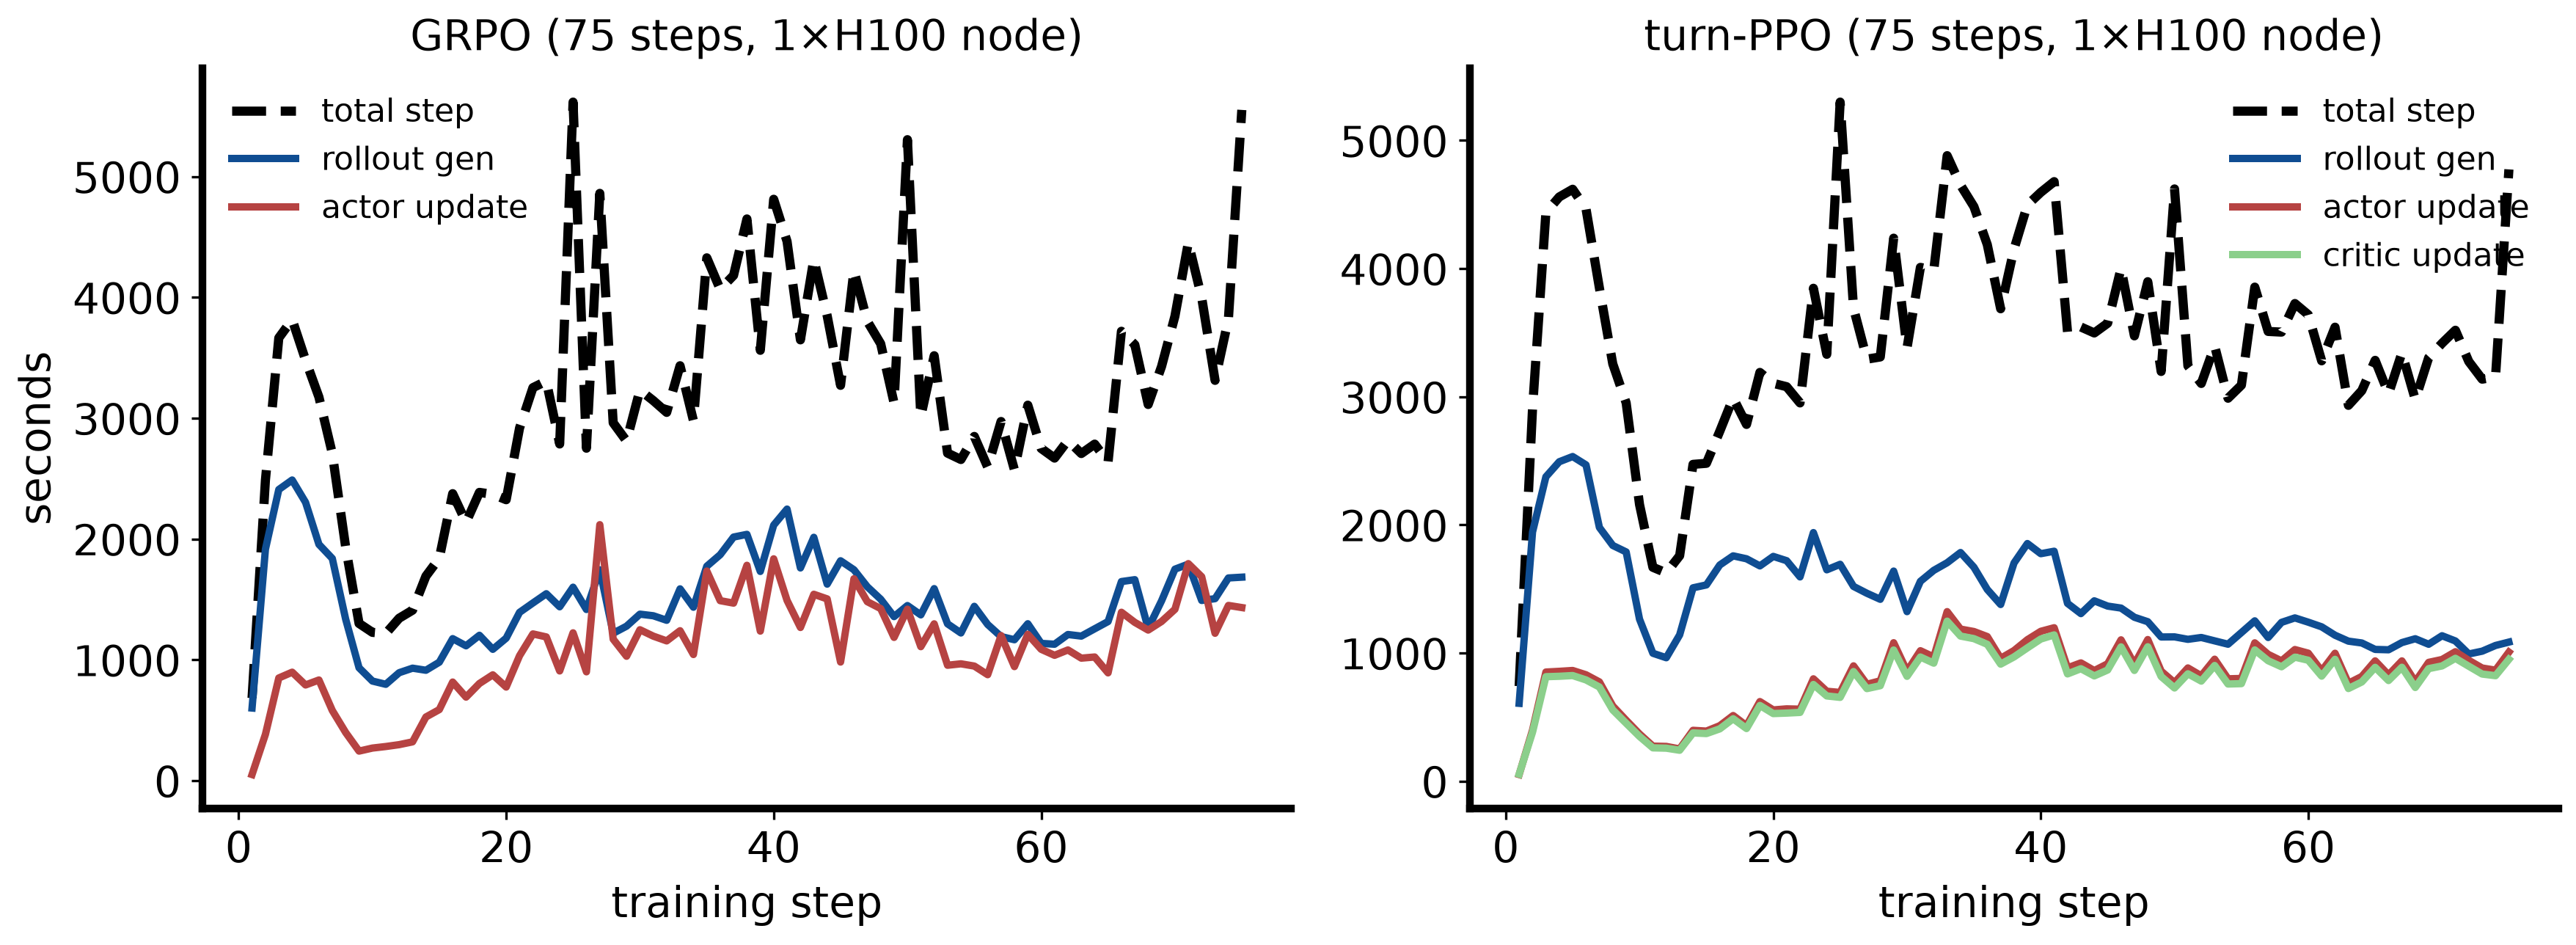
\includegraphics[width=\textwidth]{assets/fig_h100_fullrun.png}
\caption{Per-step phase times across training. GRPO's step time grows 1.6$\times$
(2{,}447\,s first-10 $\to$ 3{,}885\,s last-10): its policy inflates to $\sim$17 turns and
per-turn responses shrink, so update + logprob costs triple while gen stays flat. turn-PPO
is flat end-to-end (3{,}395\,s $\to$ 3{,}393\,s): the critic steers toward $\sim$7.5-turn
episodes, gen \emph{falls} from 1{,}930\,s to 1{,}067\,s, paying for the critic's own
$\sim$27\% overhead. Spikes are val/checkpoint steps.}
\end{figure}

\textbf{Bottlenecks (H100).} GRPO: rollout generation, 46.7\% of the run (actor update
34.3\%, logprob+ref 15.8\%). turn-PPO: the update side — actor+critic updates plus critic
forward total 50.8\%, overtaking gen (41.4\%). The single biggest lever for both remains
active-slot packing in gen (finished trajectories still generate every round).

\section{H100 vs.\ B200, position-matched steps}
\begin{table}[h]\centering\small
\begin{tabular}{lrrrr}\toprule
\multicolumn{5}{c}{\textbf{turn-PPO}, steps 1--7 mean}\\
phase & H100 s & B200 s & wall ratio & per-token\\\midrule
\matchedturnppo
\bottomrule\end{tabular}\par\vspace{0.8em}
\begin{tabular}{lrrrr}\toprule
\multicolumn{5}{c}{\textbf{GRPO}, steps 1--8 mean}\\
phase & H100 s & B200 s & wall ratio & per-token\\\midrule
\matchedgrpo
\bottomrule\end{tabular}
\caption{Position-matched phase means. H100 critic is FSDP-offloaded; B200 critic on-GPU
— that placement difference is included deliberately as ``what you would actually run''
on each hardware.}
\end{table}

\begin{figure}[h]\centering
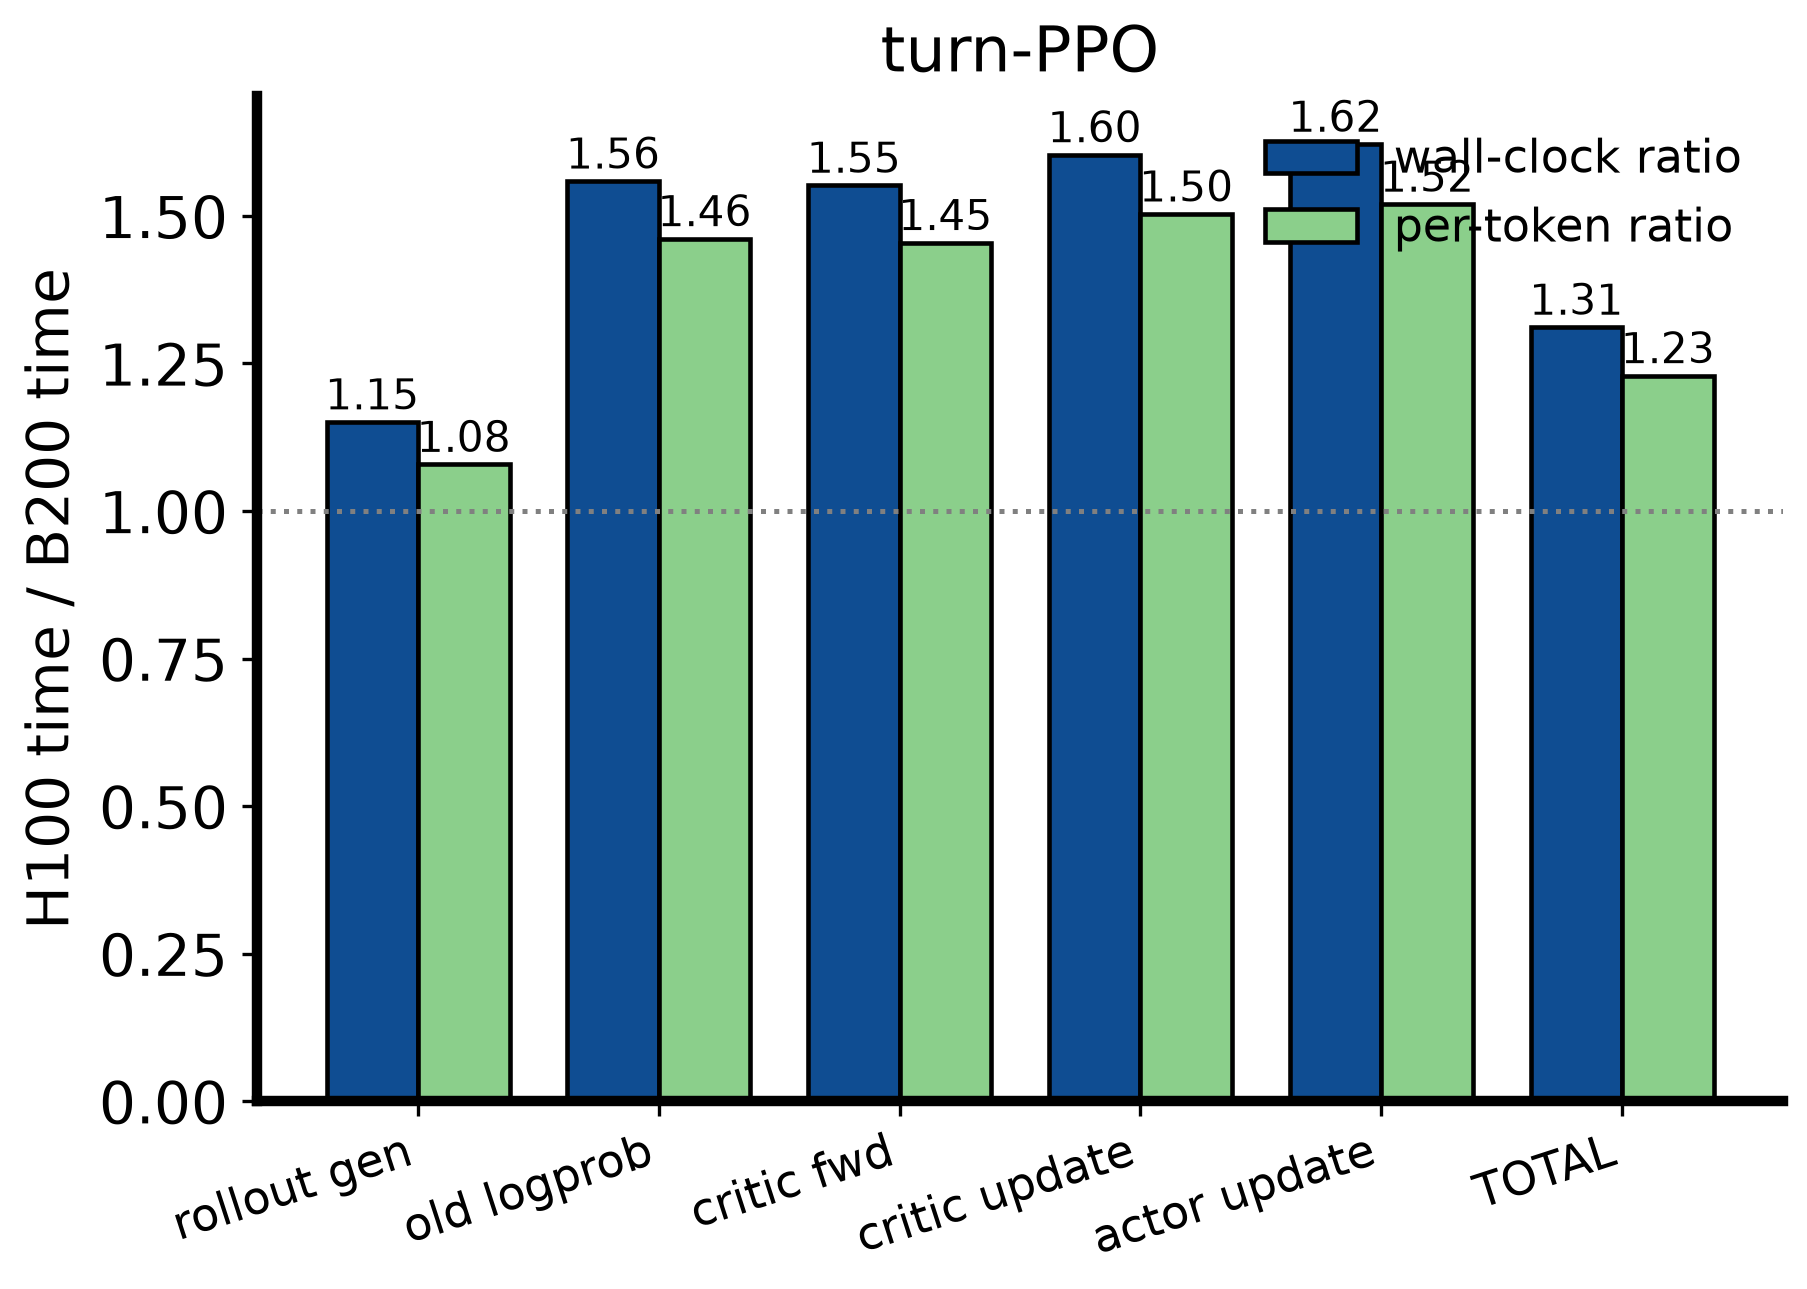
\includegraphics[width=0.98\textwidth]{assets/fig_speedup.png}
\caption{H100$\to$B200 speedup by phase (left bars wall-clock, right bars per-token).}
\end{figure}

\begin{figure}[h]\centering
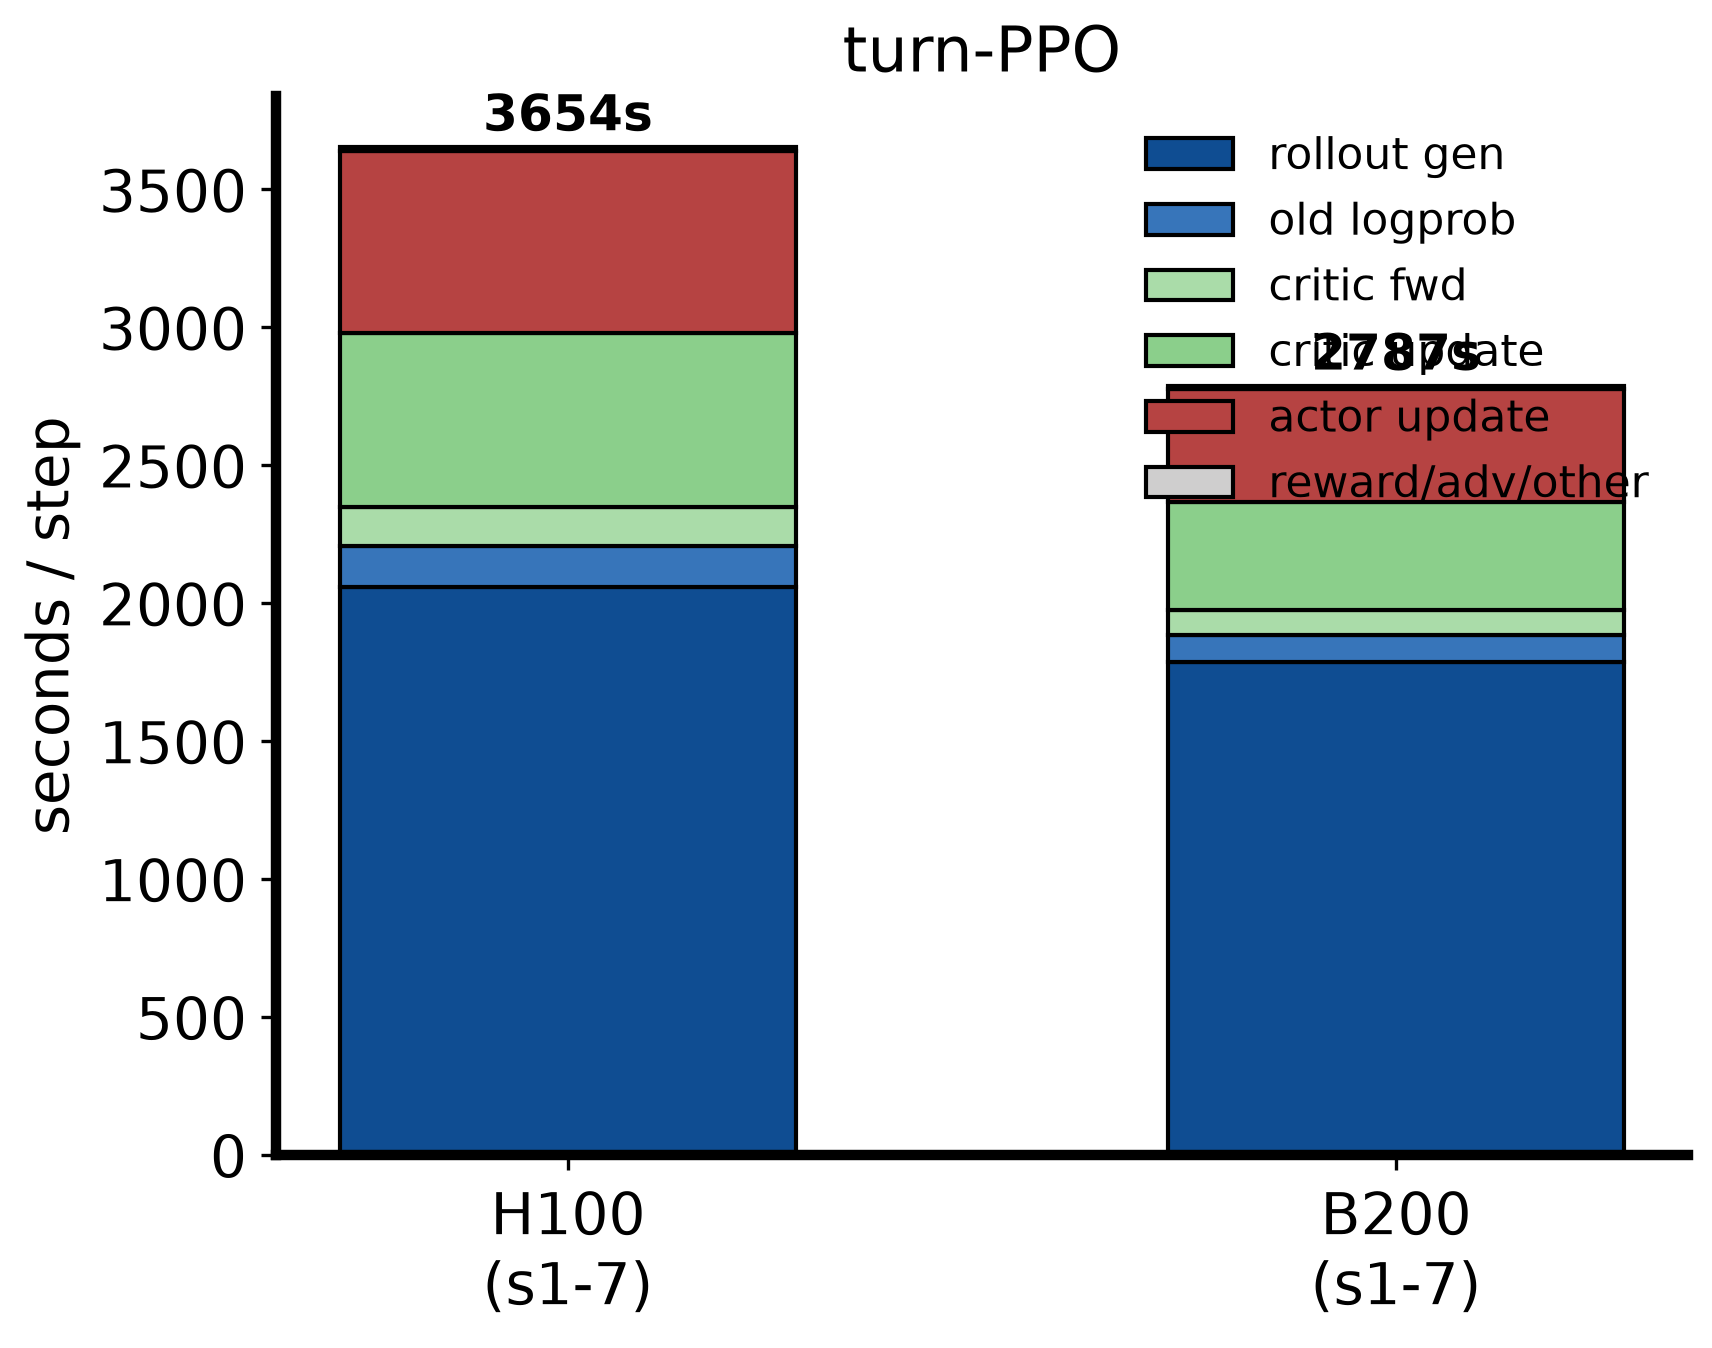
\includegraphics[width=0.9\textwidth]{assets/fig_phase_breakdown.png}
\caption{Step composition, matched steps.}
\end{figure}

\textbf{Reading.} Training-side phases (updates, logprob/values forwards) gain
$\sim$1.5--1.6$\times$ on B200 — bf16 GEMM headroom (2.1$\times$ microbench) discounted by
non-GEMM time at MFU $\approx$0.31. Generation gains only $\sim$1.1--1.2$\times$: vLLM on
sm\_100 still runs the TRITON attention backend (vendored flash-attn segfaults in CUDA-graph
capture), and decode is memory/latency-bound rather than GEMM-bound. Since gen is
41--47\% of these workloads, end-to-end lands well below the GEMM ratio.

\paragraph{Full-run estimate.} Dividing each H100 full-run phase total by its measured
per-token ratio (val/checkpoint kept at 1$\times$; identical token trajectory assumed):
75-step turn-PPO $\approx$ \extrapturnppo; 75-step GRPO $\approx$ \extrapgrpo. This matches
the 1.53$\times$ end-to-end measured in the 2026-08-01 four-cycle pilot within its noise.
An 8-step pilot cannot capture policy-drift effects on gen; treat these as
$\pm$10\% estimates.

\section{Cost perspective}
At equal node counts B200 shortens a 75-step arm from $\sim$3 days to $\sim$2. Caveats
that are operational, not performance: cross-region HDFS staging (25--360\,MB/s, $\sim$25
min/pod), no faiss (torch retrieval server), no egress (wandb/HF offline), and the
LD\_PRELOAD libcuda fix. All are scripted in \texttt{p8b\_b200\_prof\_worker.sh}.

\section{2$\times$H100: measured verdict — not runnable on current resources}
Two independent blockers, both verified:
\begin{enumerate}\itemsep2pt
  \item \textbf{Workspace workers} (our queue): no \texttt{/dev/infiniband}; NCCL falls back
  to socket transport and its ephemeral data ports are firewalled — the first cross-node
  allreduce fails with \texttt{ncclRemoteError} (probe \texttt{nccl\_probe.sh}, 2026-08-03).
  Rendezvous and Ray cluster formation work; only collectives fail.
  \item \textbf{Arnold training jobs}: per the platform's resource-queue manual, RDMA
  requires a \emph{minipod}-tagged queue; the \texttt{mlsys\_inference} group has none
  (checked 2026-08-04). Best case is socket NCCL at single-digit GB/s vs.\ 400\,GB/s
  NVLink intra-node — with updates at 34--51\% of step time, 2 nodes would be slower than 1.
\end{enumerate}
\textbf{Unblock:} a minipod-bound H100 queue for \texttt{mlsys\_inference} (the platform's
own term for RDMA-provisioned training queues). A ready-to-submit 2-node probe job
(\texttt{scripts/asearcher/mlx\_nccl\_probe\_job.yaml}) verifies transport the day such a
queue exists. No honest scaling-efficiency number can be produced before then.

\section*{Reproduction}
\texttt{python mine\_timings.py --out assets/timings.json grpo\_h100=... turn\_ppo\_h100=...
b200=...} then \texttt{python make\_figures.py} and \texttt{tectonic hw\_algo\_profiling.tex}.
Raw per-step data: \texttt{assets/timings.json}; computed numbers:
\texttt{assets/computed\_tables.json}.

\end{document}
